\documentclass[11pt]{article}

\usepackage[margin=1in]{geometry}
\usepackage[T1]{fontenc}
\usepackage[utf8]{inputenc}
\usepackage{amsmath,amssymb}
\usepackage{graphicx}
\usepackage{booktabs,array}
\usepackage{float}
\usepackage{xcolor}
\usepackage{hyperref}
\usepackage{caption}
\usepackage{enumitem}
\hypersetup{colorlinks=true, linkcolor=blue!60!black, urlcolor=blue!60!black}
\setlength{\parindent}{0pt}
\setlength{\parskip}{0.6em}
\setlist[itemize]{leftmargin=1.25em, itemsep=0.2em, topsep=0.3em}

\newcommand{\commentarybox}[1]{%
  \vspace{0.4em}
  \noindent\fcolorbox{black}{yellow!8}{%
    \parbox{\dimexpr\linewidth-2\fboxsep-2\fboxrule\relax}{%
      \textbf{Personal commentary to add:} #1
      \vspace{1.8cm}
    }%
  }
}

\newcommand{\sourcebox}[1]{%
  \noindent\fcolorbox{black}{gray!8}{%
    \parbox{\dimexpr\linewidth-2\fboxsep-2\fboxrule\relax}{#1}%
  }
}

\title{How AI Coding Agents Supported This Raman-Suppression Research Project}
\author{Fiber Raman Suppression Project}
\date{Presentation companion draft: 2026-04-27}

\begin{document}
\maketitle

\begin{abstract}
This short note explains how AI coding agents were used in the Raman-suppression
project.  The main point is not that AI ``did the research.''  The useful
framing is that AI agents became a research accelerator: they helped search a
large codebase, draft and refactor code, generate figures, compile documents,
run checks, and organize results, while the human researcher chose the
questions, judged the claims, and decided what was scientifically convincing.
The workflow worked best when agents were given clear context, narrow tasks,
real verification loops, and strict documentation standards.
\end{abstract}

\section*{Status}
\sourcebox{\textbf{Purpose:} presentation support.  This is not a physics
result note.  It is a compact explanation of the research workflow and should
be edited with the author's personal experience before being presented.}

\section{The Core Framing}

The simplest honest explanation is:

\begin{quote}
I used AI agents as research assistants, coding partners, documentation editors,
and verification checkers.  I did not treat them as an authority on the science.
\end{quote}

That distinction matters.  The agents were useful because the project had many
moving parts: Julia simulation code, Python tooling, LaTeX reports, result
images, burst-compute runs, gradient checks, and many months of notes.  AI was
most helpful when the work could be turned into a loop: gather context, make a
bounded change, run checks, inspect artifacts, and summarize what changed.

\begin{figure}[H]
\centering
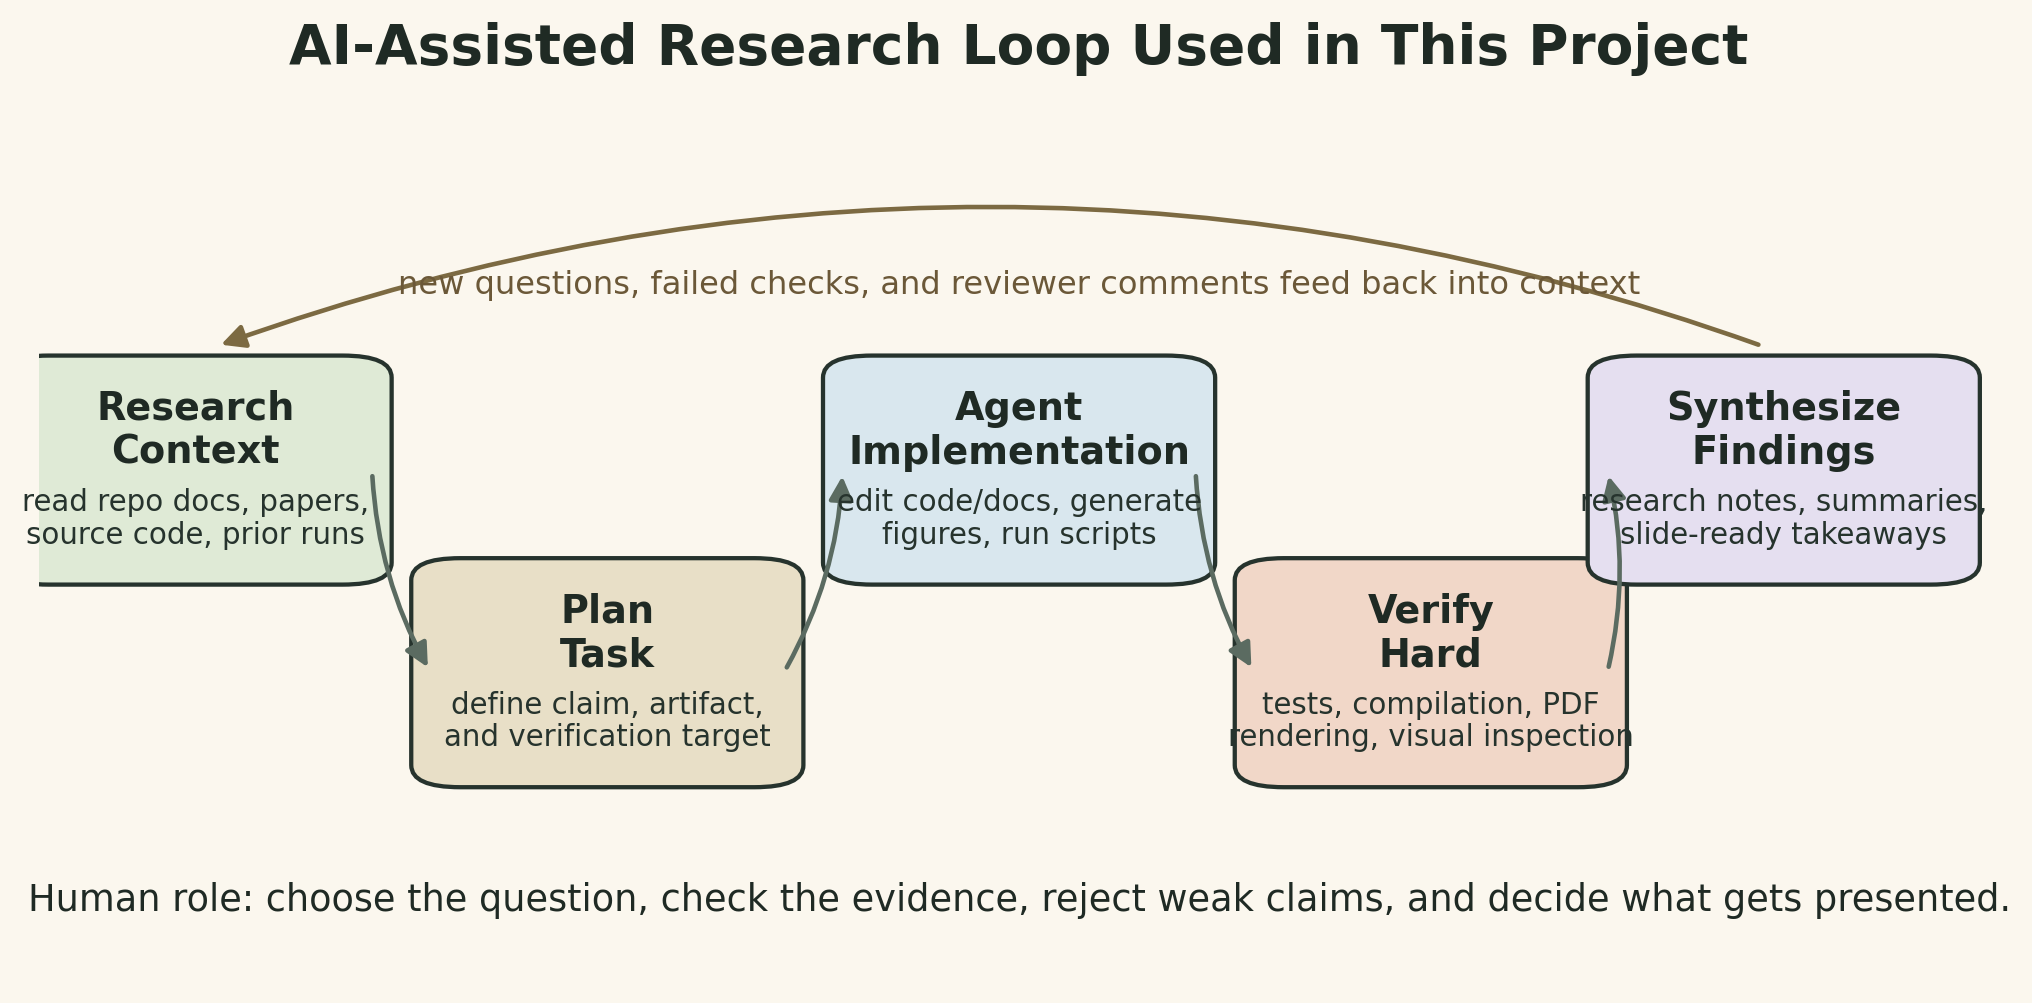
\includegraphics[width=0.95\linewidth]{figures/project_ai_research_loop.png}
\caption{The practical loop used throughout this project.  AI helped move
through the loop faster, but failed checks and unclear claims still had to
come back to the human researcher.}
\end{figure}

\commentarybox{Add one concrete story here: a moment where an agent saved time,
and a moment where you had to push back because the answer was too shallow,
wrong, or overconfident.}

\section{What The Outside Agentic-Coding Literature Says}

The current agentic-coding discussion has a common theme: the human role shifts
from typing every line to designing the environment, setting intent, and
building feedback loops.  OpenAI describes this as harness engineering: humans
steer and agents execute, with constraints and feedback loops doing much of the
quality control \cite{openai-harness}.  OpenAI's internal Codex guidance also
emphasizes code understanding, refactoring, performance work, test coverage,
issue-style prompts, persistent repository instructions, and task queues
\cite{openai-codex}.

Peter Steinberger's writing is especially relevant because it is practical and
opinionated.  The strongest takeaway from his agentic-engineering posts is not
``use many agents blindly.''  It is to develop intuition for task size, blast
radius, when to interrupt an agent, when to ask for options, and when to rely
on tests and fast feedback instead of manually reading every line
\cite{steinberger-talk}.  His workflow posts also stress a terminal-first setup,
small tasks, plan review for bigger changes, and refactoring as routine
maintenance rather than an afterthought \cite{steinberger-workflow}.

The more conservative best-practice literature adds the necessary caution:
developers remain accountable, generated code must be understood and verified,
security boundaries matter, and checkpoints make mistakes reversible
\cite{agentic-principles,openai-governance}.

\begin{figure}[H]
\centering
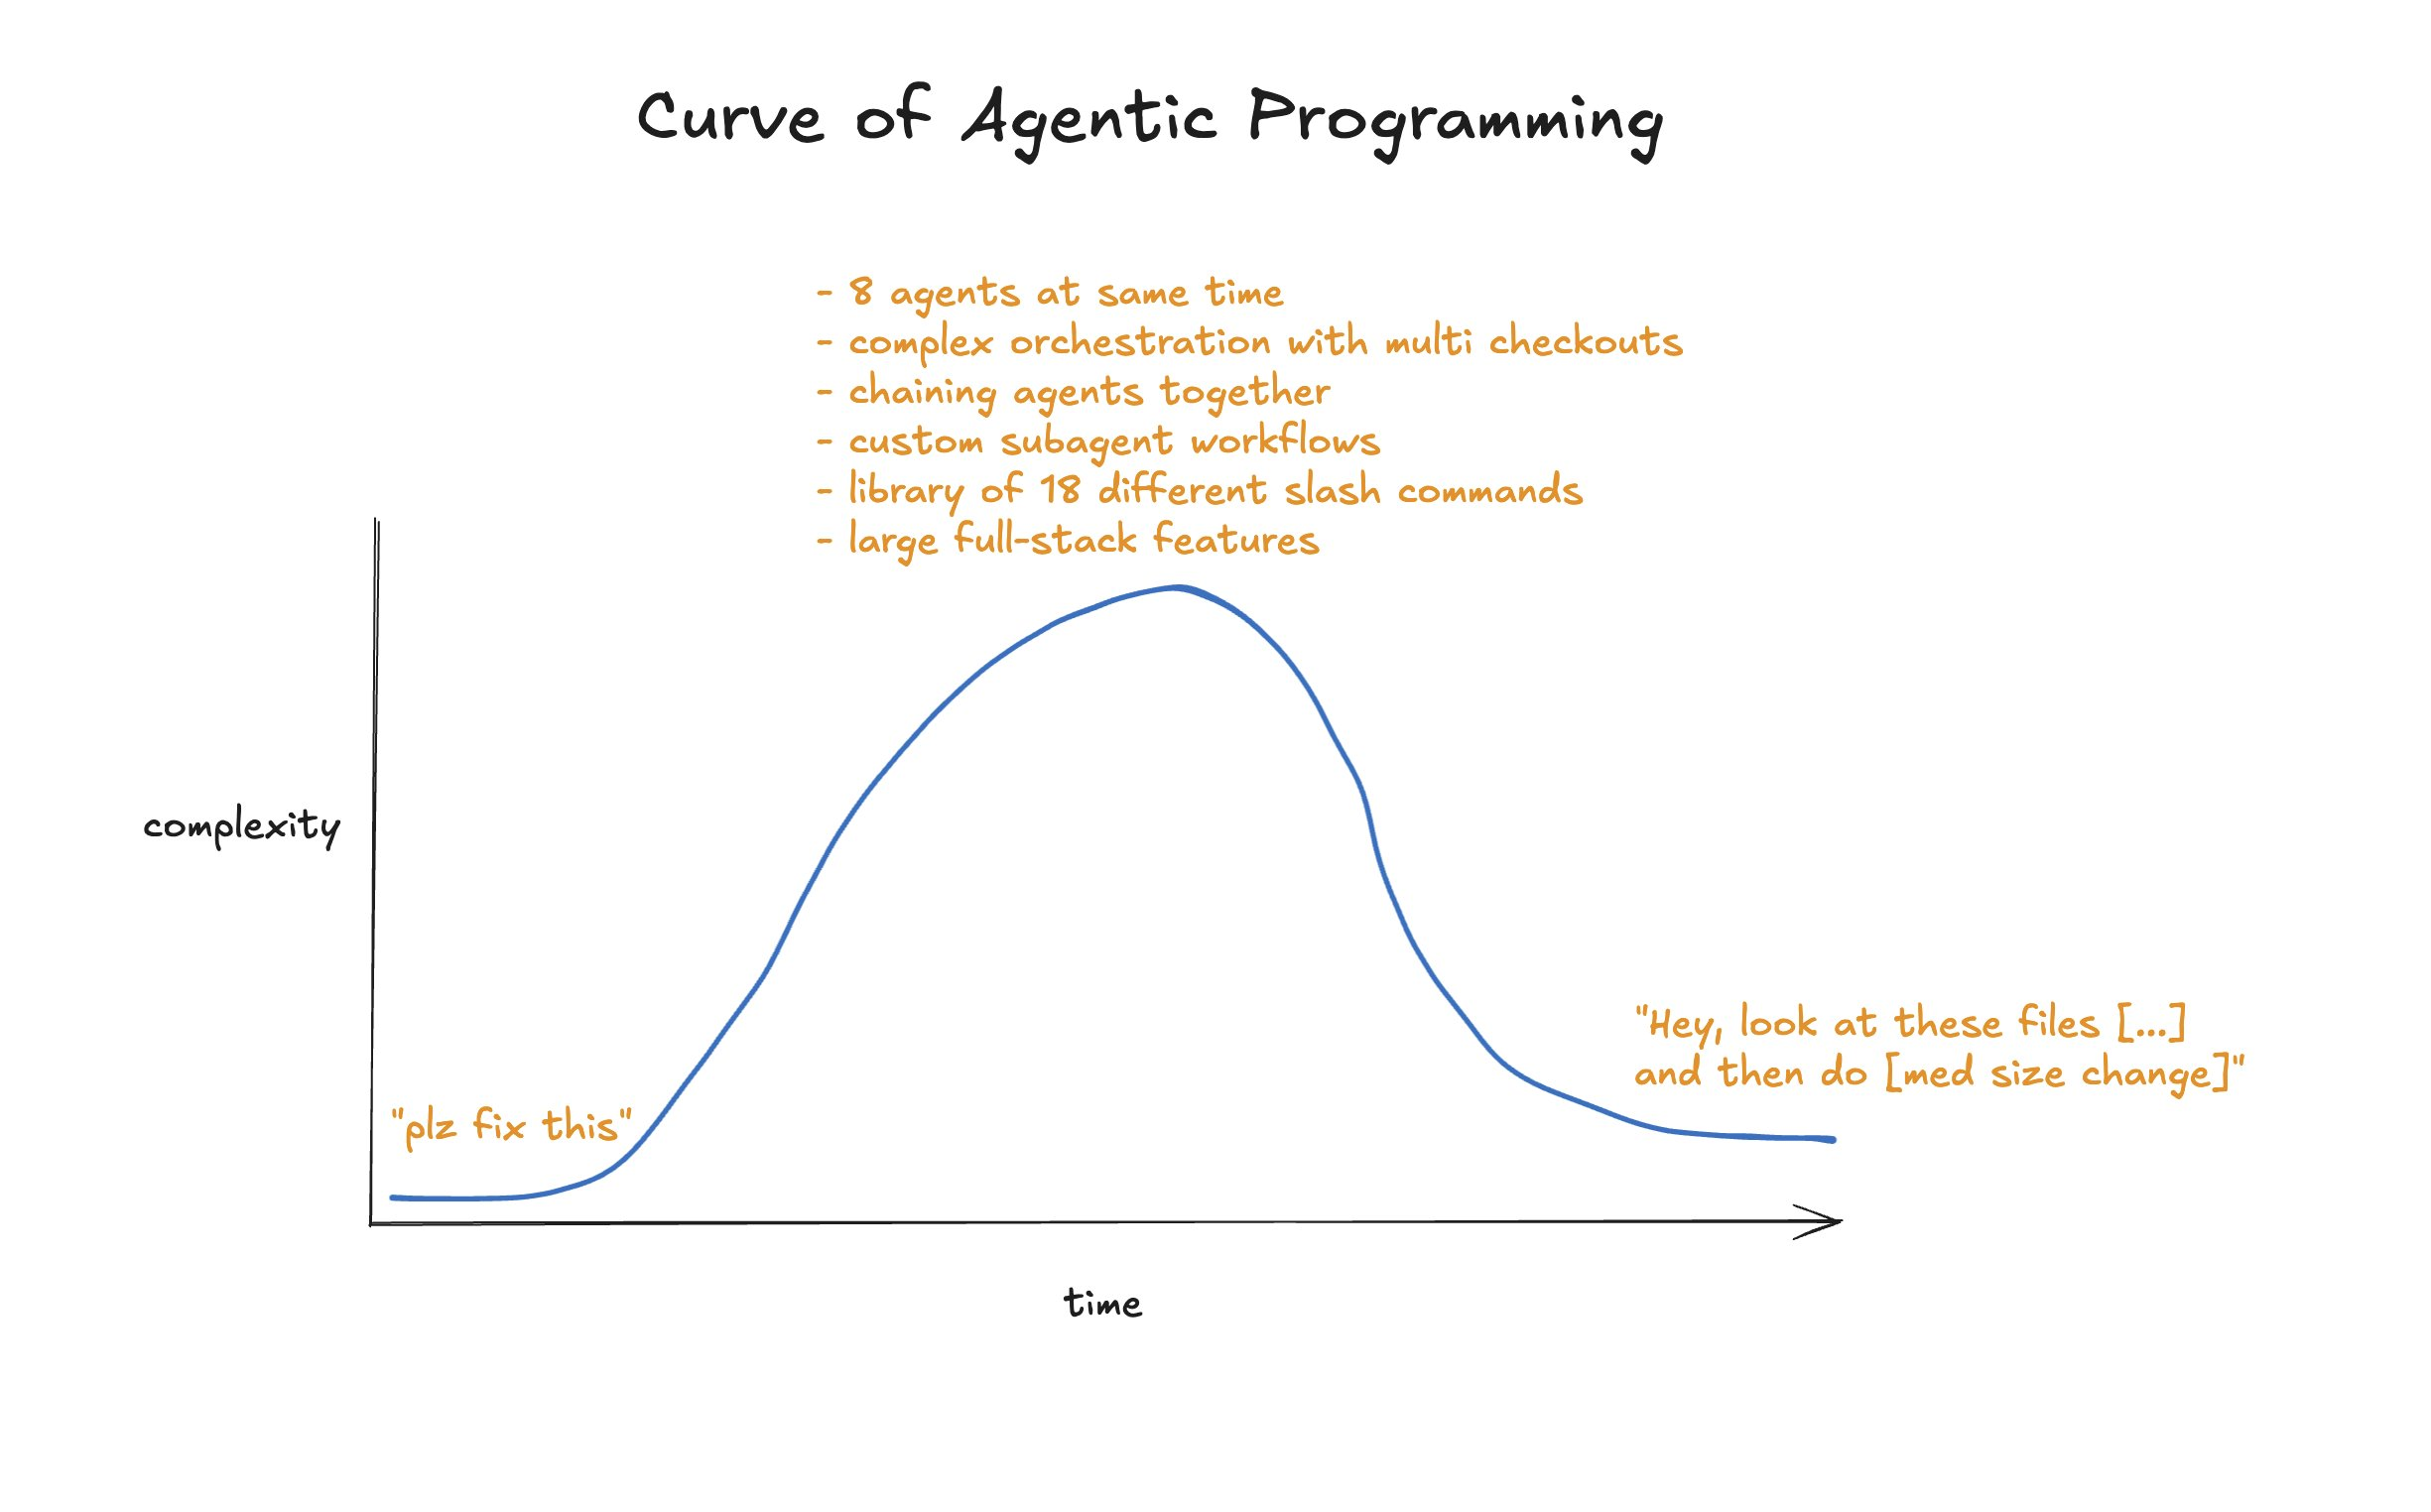
\includegraphics[width=0.82\linewidth]{figures/steinberger_agentic_curve.jpg}
\caption{Peter Steinberger's ``Curve of Agentic Programming'' image, reused
from steipete.me.  The useful lesson for this project is that complexity should
not be added for its own sake: small direct prompts, visible terminal work, and
fast feedback often beat elaborate orchestration.}
\end{figure}

\commentarybox{Add whether this matches your experience.  Did the project work
better when prompts were short and direct?  Did large vague tasks fail more
often?  Mention one example.}

\section{How This Applied To The Raman Project}

This project was not a normal app-development project.  It mixed numerical
physics, optimization, plotting, documentation, and compute operations.  That
changed how AI was useful.

\begin{center}
\small
\begin{tabular}{>{\raggedright\arraybackslash}p{0.28\linewidth}
                >{\raggedright\arraybackslash}p{0.31\linewidth}
                >{\raggedright\arraybackslash}p{0.31\linewidth}}
\toprule
\textbf{Project need} & \textbf{Agent contribution} & \textbf{Human check} \\
\midrule
Understand old work & Search docs, summarize prior runs, map files to claims &
Decide which old findings were still trustworthy. \\
Implement scripts & Edit Julia/Python/LaTeX, add helpers, organize outputs &
Inspect diffs, run tests, reject unsafe changes. \\
Verify math & Draft derivations, compare code paths, propose finite-difference
tests & Re-derive important equations and ask for blind verification. \\
Create figures & Generate diagrams, copy standard images, assemble PDFs &
Open rendered PDFs and inspect image overlap, captions, and readability. \\
Prepare presentation docs & Turn scattered findings into note structure &
Choose the story, tone, and what should be emphasized to the lab. \\
\bottomrule
\end{tabular}
\end{center}

\begin{figure}[H]
\centering
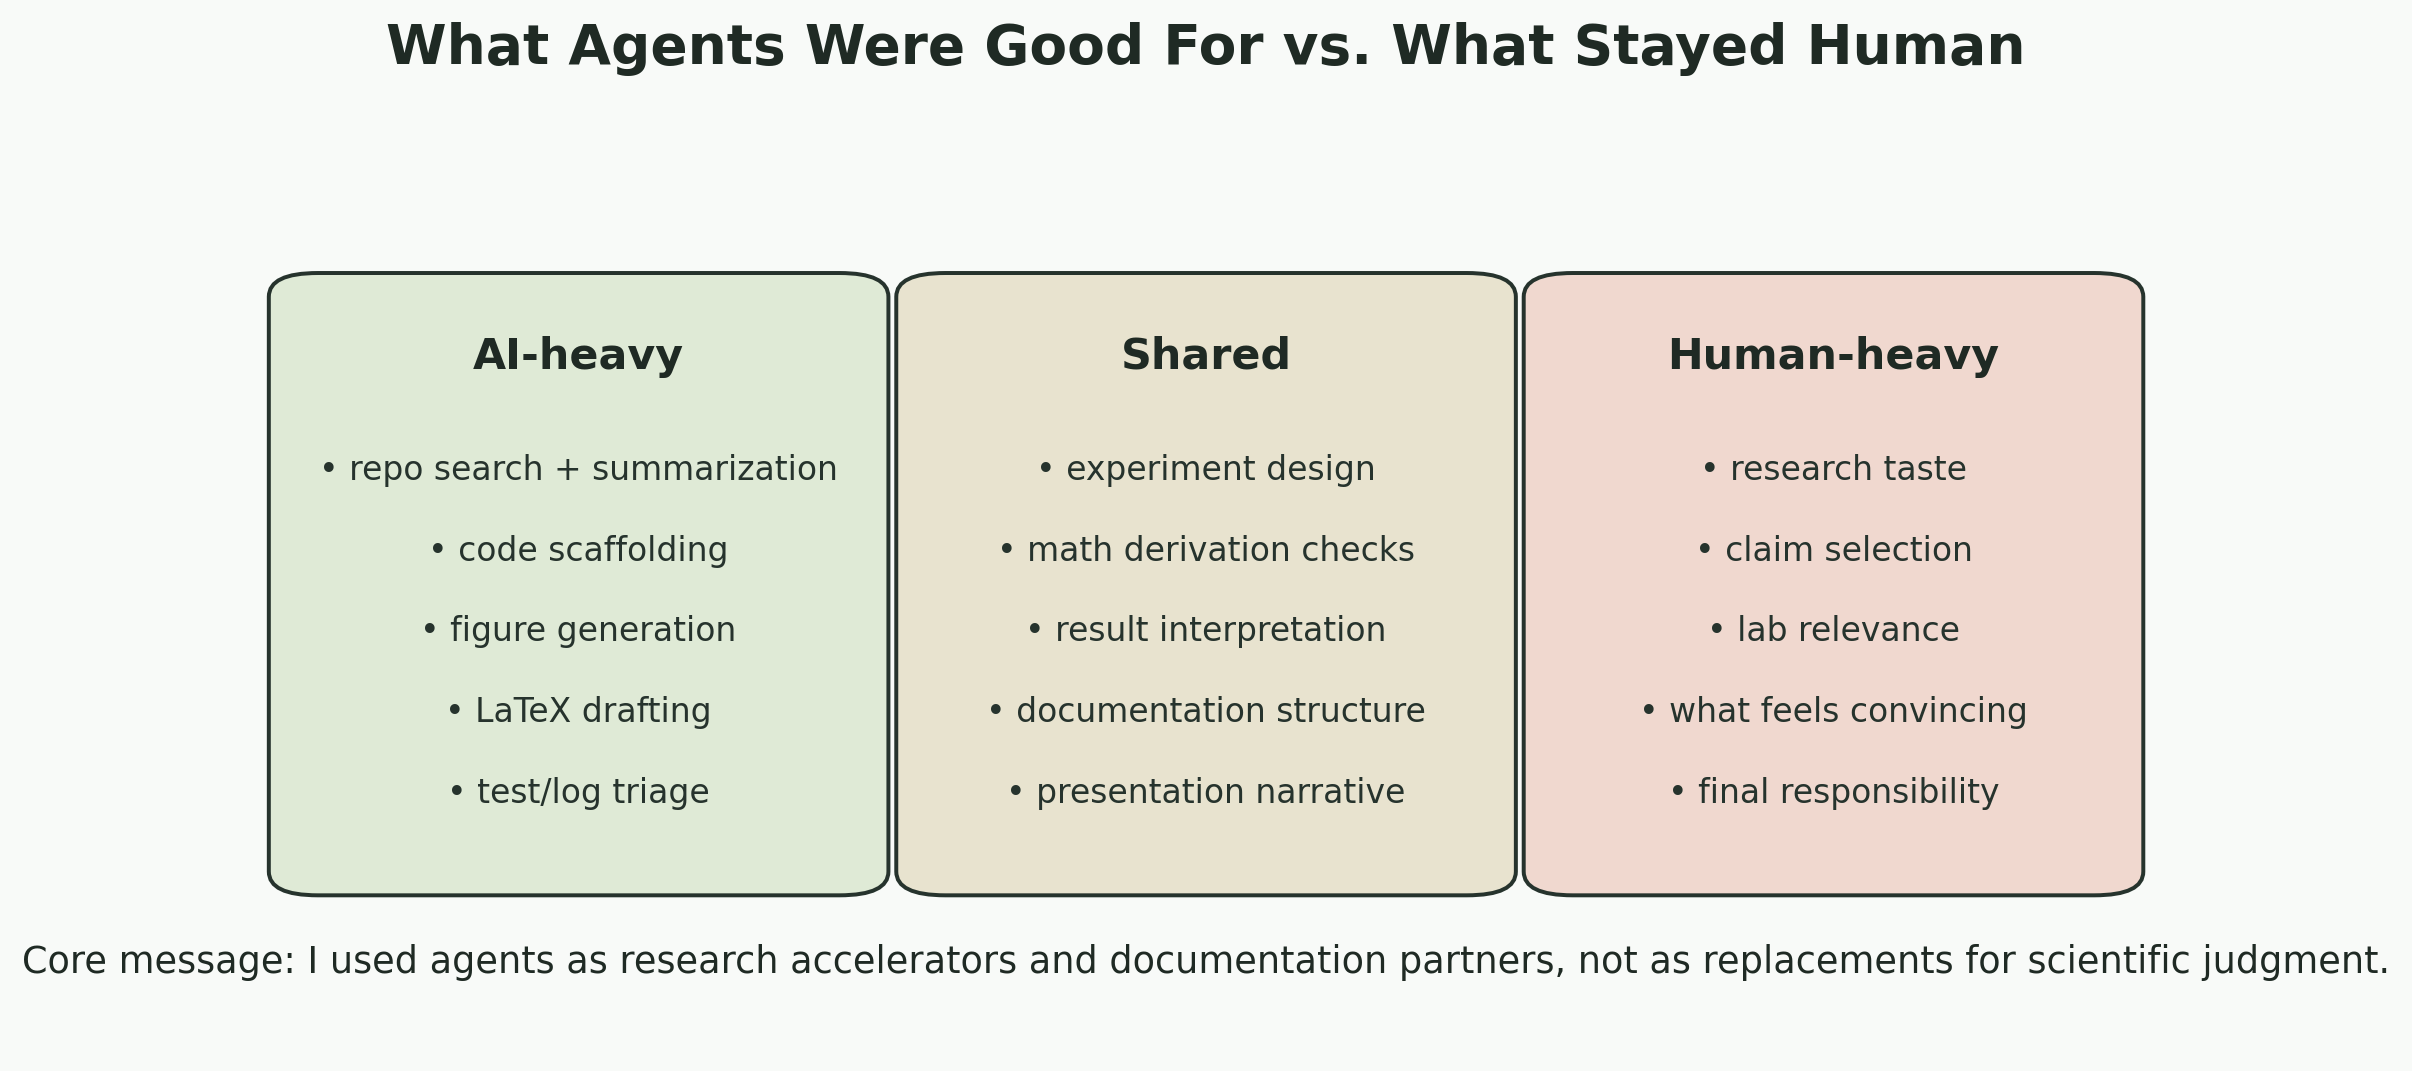
\includegraphics[width=0.92\linewidth]{figures/agent_human_responsibility_map.png}
\caption{Division of labor.  The productive workflow was not ``AI versus
human.''  It was assigning mechanical, search-heavy, and formatting-heavy work
to agents while keeping scientific judgment with the researcher.}
\end{figure}

\commentarybox{Add your own examples in each column: one coding task, one
documentation task, one math/verification task, and one presentation task.}

\section{CS Design Principles That Made AI Engineering Work}

One lesson from the project is that AI agents do better when the codebase is
designed with old-school computer science discipline.  The new tool is AI, but
the enabling ideas are not new: abstraction, modularity, contracts, testing,
and observability.

\begin{figure}[H]
\centering
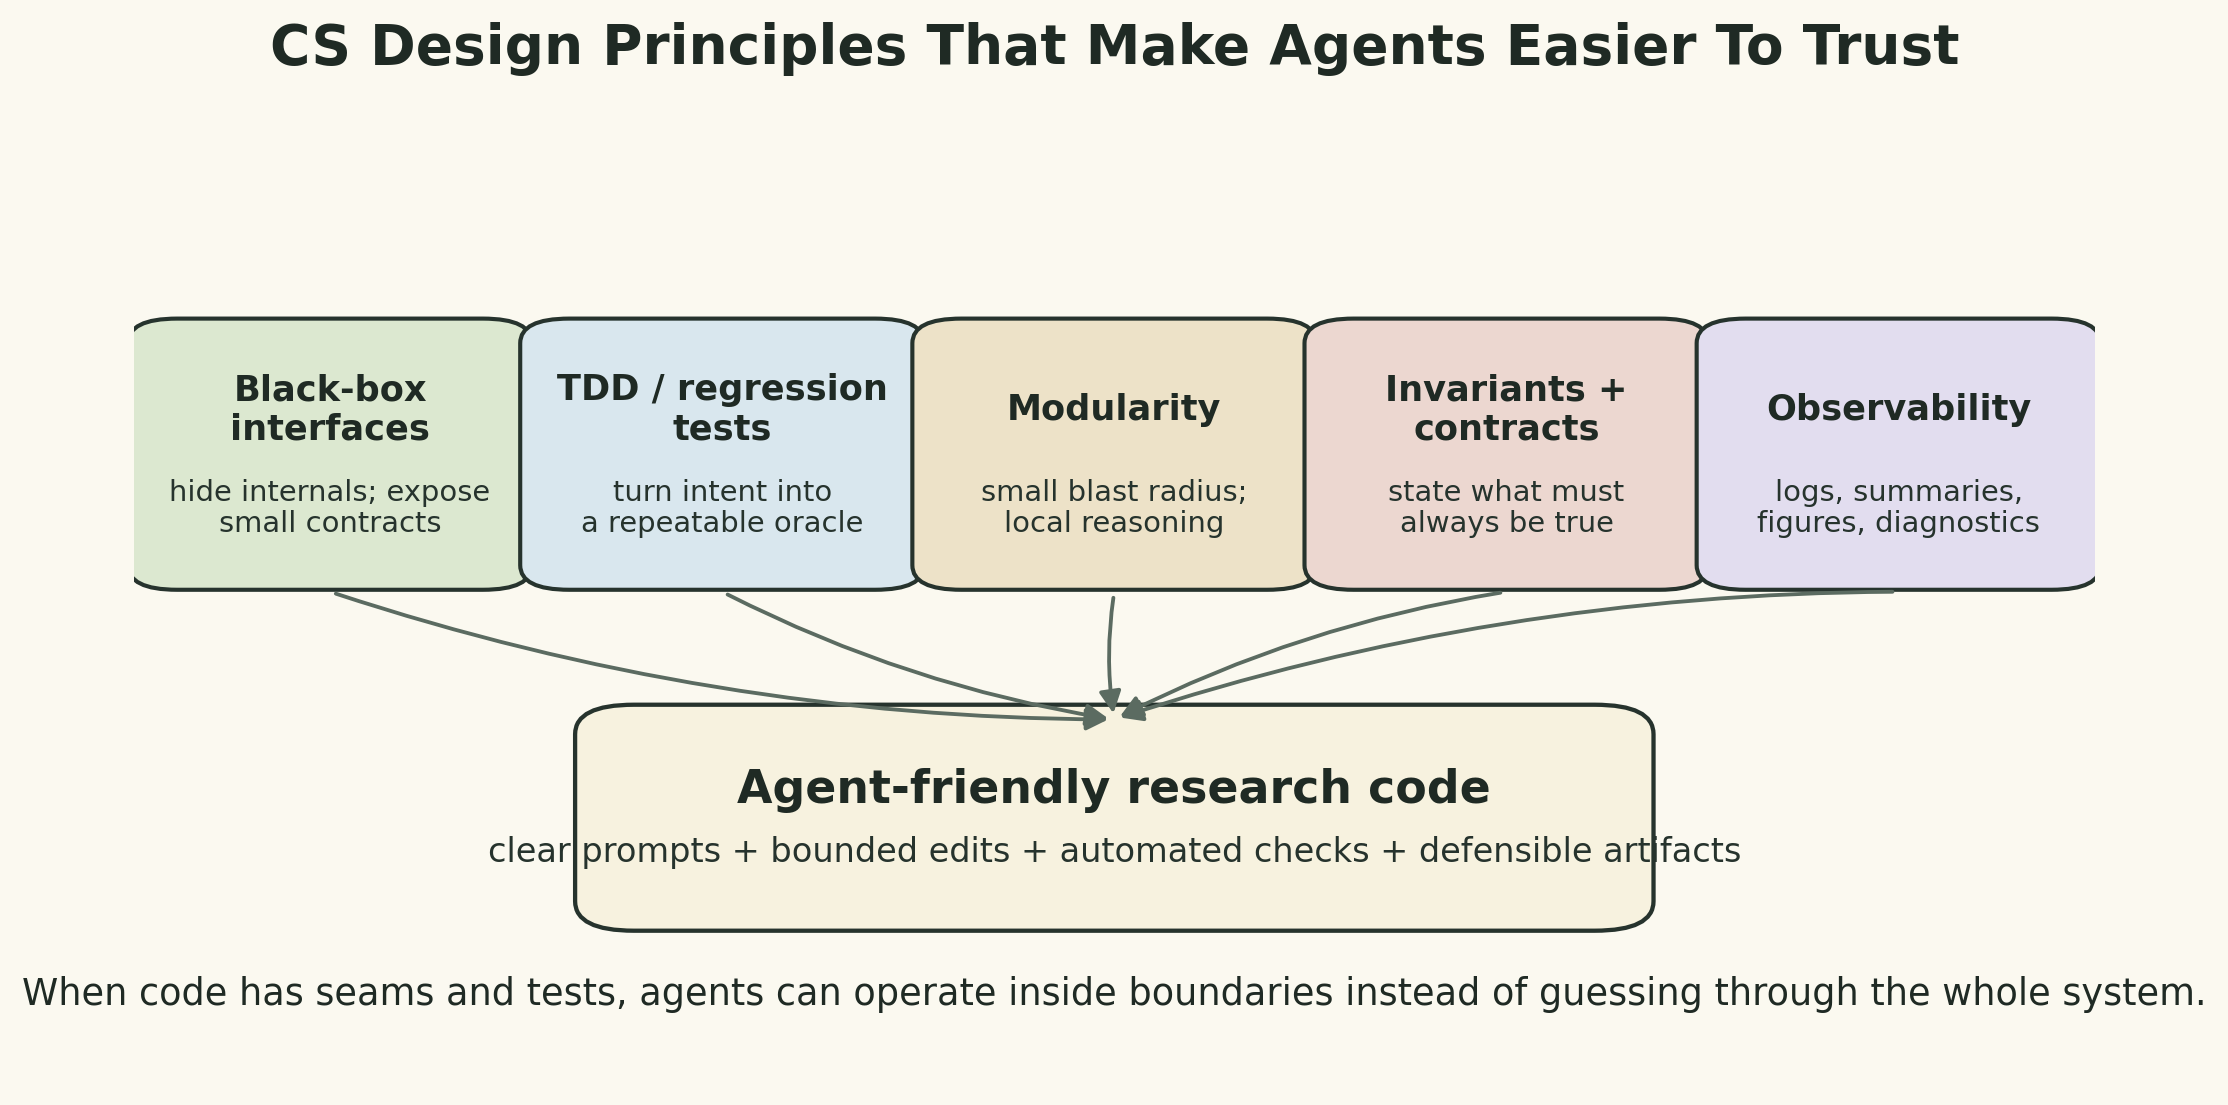
\includegraphics[width=0.94\linewidth]{figures/cs_principles_for_ai_engineering.png}
\caption{Fundamental CS principles made the codebase more agent-friendly.
Agents are much more useful when they can work inside clean boundaries and then
prove their work with tests, diagnostics, and artifacts.}
\end{figure}

\subsection*{Black-Box Design and Information Hiding}

Black-box design means a module exposes a small, stable interface while hiding
its internal implementation.  This is the same core idea as Parnas's
information-hiding criterion for modular decomposition: modules should hide
design decisions that are likely to change \cite{parnas1972}.  For AI agents,
that matters because a clean interface gives the model a smaller surface to
reason about.

In this project, a good black-box boundary looked like:
\begin{center}
\small
\begin{tabular}{c}
\texttt{save\_standard\_set(problem, result, tag)} \\
\(\Downarrow\) \\
phase profile, phase diagnostic, optimized evolution, control evolution
\end{tabular}
\end{center}
The agent did not need to re-understand every plotting detail each time.  It
only needed to know the contract: optimized runs must produce the standard
image set.

\subsection*{Test-Driven Development}

TDD is useful with agents because it turns an English request into an executable
oracle.  Kent Beck's classic formulation is to write a failing test, make it
pass, then refactor \cite{beck2002}.  In an AI workflow, that pattern becomes
even more important because the agent can generate plausible code quickly, but
plausible code is not the same thing as correct code.

For this project, the equivalent of TDD included:
\begin{itemize}
\item finite-difference gradient checks before trusting adjoints;
\item PDF compilation and page rendering before trusting LaTeX;
\item standard image generation before trusting an optimization run;
\item source-text scans before trusting that public docs were outward-facing;
\item regression tests before treating infrastructure changes as safe.
\end{itemize}

\subsection*{Contracts, Invariants, and Preconditions}

Design-by-contract thinking says a component should state what it expects, what
it guarantees, and what must remain invariant \cite{meyer1997}.  This maps
directly onto AI-assisted research code.  The agent should know the preconditions
for a task, the postconditions that prove it finished, and the invariants it
must not break.

Examples from the project:
\begin{itemize}
\item Heavy simulations must run on the burst machine, not the editing host.
\item A run that produces an optimized phase must leave standard images.
\item A public note must compile to PDF and be visually inspected.
\item A reduced-basis gradient must obey \(\nabla_c J = B^T\nabla_\phi J\).
\item A result is not final if it only has a plot and no provenance.
\end{itemize}

\subsection*{Observability and Reproducibility}

Agents need feedback.  In ordinary software, that means logs, errors, tests,
and traces.  In this research project, it also meant plots, convergence tables,
energy drift, edge fractions, rendered PDFs, and result summaries.  Good
observability made it possible to ask an agent not just ``did it run?'' but
``what happened, where did it fail, and what evidence changed?''

\commentarybox{Add your own CS-principles example here.  Suggested prompt:
``The reason black-box design/TDD mattered in my project was ...''  A strong
example would be standard images, gradient checks, or the reduced-basis map.}

\section{Techniques That Worked}

\subsection*{1. Persistent Project Rules}

The repo used persistent instructions such as \texttt{AGENTS.md},
\texttt{CLAUDE.md}, current-agent context files, and quality standards.  This
made agents more reliable because they did not have to infer the workflow from
scratch every session.

In this project, persistent rules mattered for practical reasons:
\begin{itemize}
\item heavy simulations belonged on the burst machine, not the editing host;
\item public docs belonged in \texttt{docs/}, while agent notes belonged in
\texttt{agent-docs/};
\item every result with an optimized phase needed standard images;
\item PDFs had to be compiled, rendered, and visually inspected.
\end{itemize}

\subsection*{2. Small Tasks With Clear Blast Radius}

Steinberger's ``blast radius'' framing is useful: before delegating to an
agent, estimate how many files and assumptions the change touches
\cite{steinberger-talk}.  Small tasks are easier to review and easier to
recover from.  Large tasks are possible, but they need stronger plans, tests,
and checkpoints.

\subsection*{3. Ask For Options Before Changes}

For uncertain work, a good pattern was:
\begin{quote}
Read the relevant files, summarize the options, and do not edit yet.
\end{quote}
This prevented premature code changes and made the agent expose its assumptions.
It was especially useful for numerical methods, result interpretation, and
paper-style documentation.

\subsection*{4. Close The Loop With Real Checks}

The agents became much more useful when every task had an external check:
\begin{itemize}
\item run tests or finite-difference checks for code;
\item compile LaTeX for docs;
\item render PDFs and inspect pages for layout;
\item compare equations against independent derivations;
\item visually inspect standard result images instead of trusting filenames.
\end{itemize}

\begin{figure}[H]
\centering
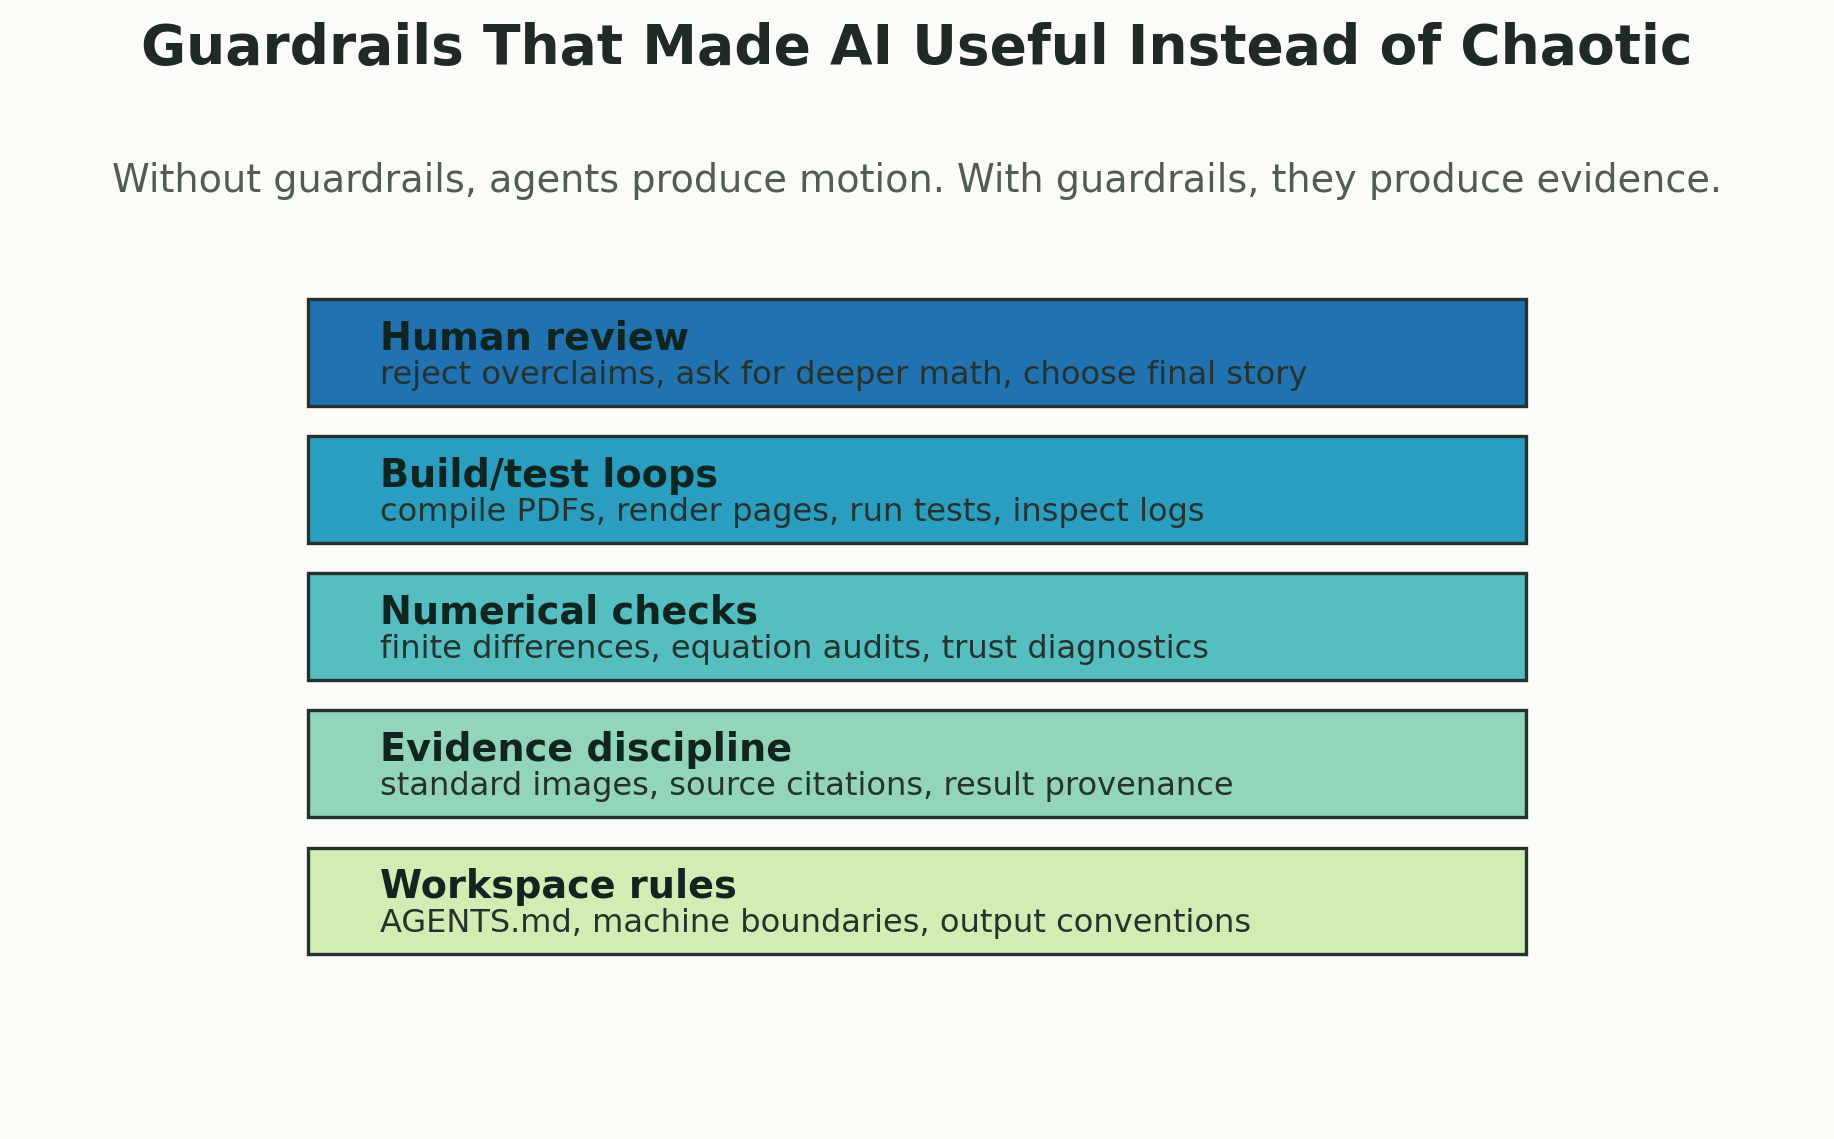
\includegraphics[width=0.88\linewidth]{figures/agent_guardrail_stack.png}
\caption{The guardrail stack.  The most important lesson is that agents are
powerful but not self-validating.  They need tests, source checks, visual
inspection, and human review.}
\end{figure}

\subsection*{5. Use Images As Context}

Modern coding agents can use screenshots and generated plots as context.
Steinberger explicitly points out that screenshots can quickly communicate UI
or visual problems \cite{steinberger-talk}.  In this project, that translated
to a rule for research notes: result images had to be included, paired, and
viewed after PDF compilation.  This caught real issues, such as overlapping
plot text or badly formatted tables.

\subsection*{6. Empathy For The Model}

One of Steinberger's most useful points is what he calls empathy for the model:
before blaming the model, ask what context it actually has available
\cite{steinberger-talk}.  A human researcher may remember months of decisions,
failed runs, preferred figure styles, and professor expectations.  The model
does not automatically know that.  It sees the prompt, the files it is told to
read, the tools it can call, and whatever constraints are written down.

In practice, model empathy meant writing prompts and repo rules that answered:
\begin{itemize}
\item What files should the model read first?
\item What is the real goal, not just the immediate edit?
\item What examples show the desired quality bar?
\item What terms, claims, or artifacts should be avoided?
\item How should the model prove the task is complete?
\end{itemize}

\begin{figure}[H]
\centering
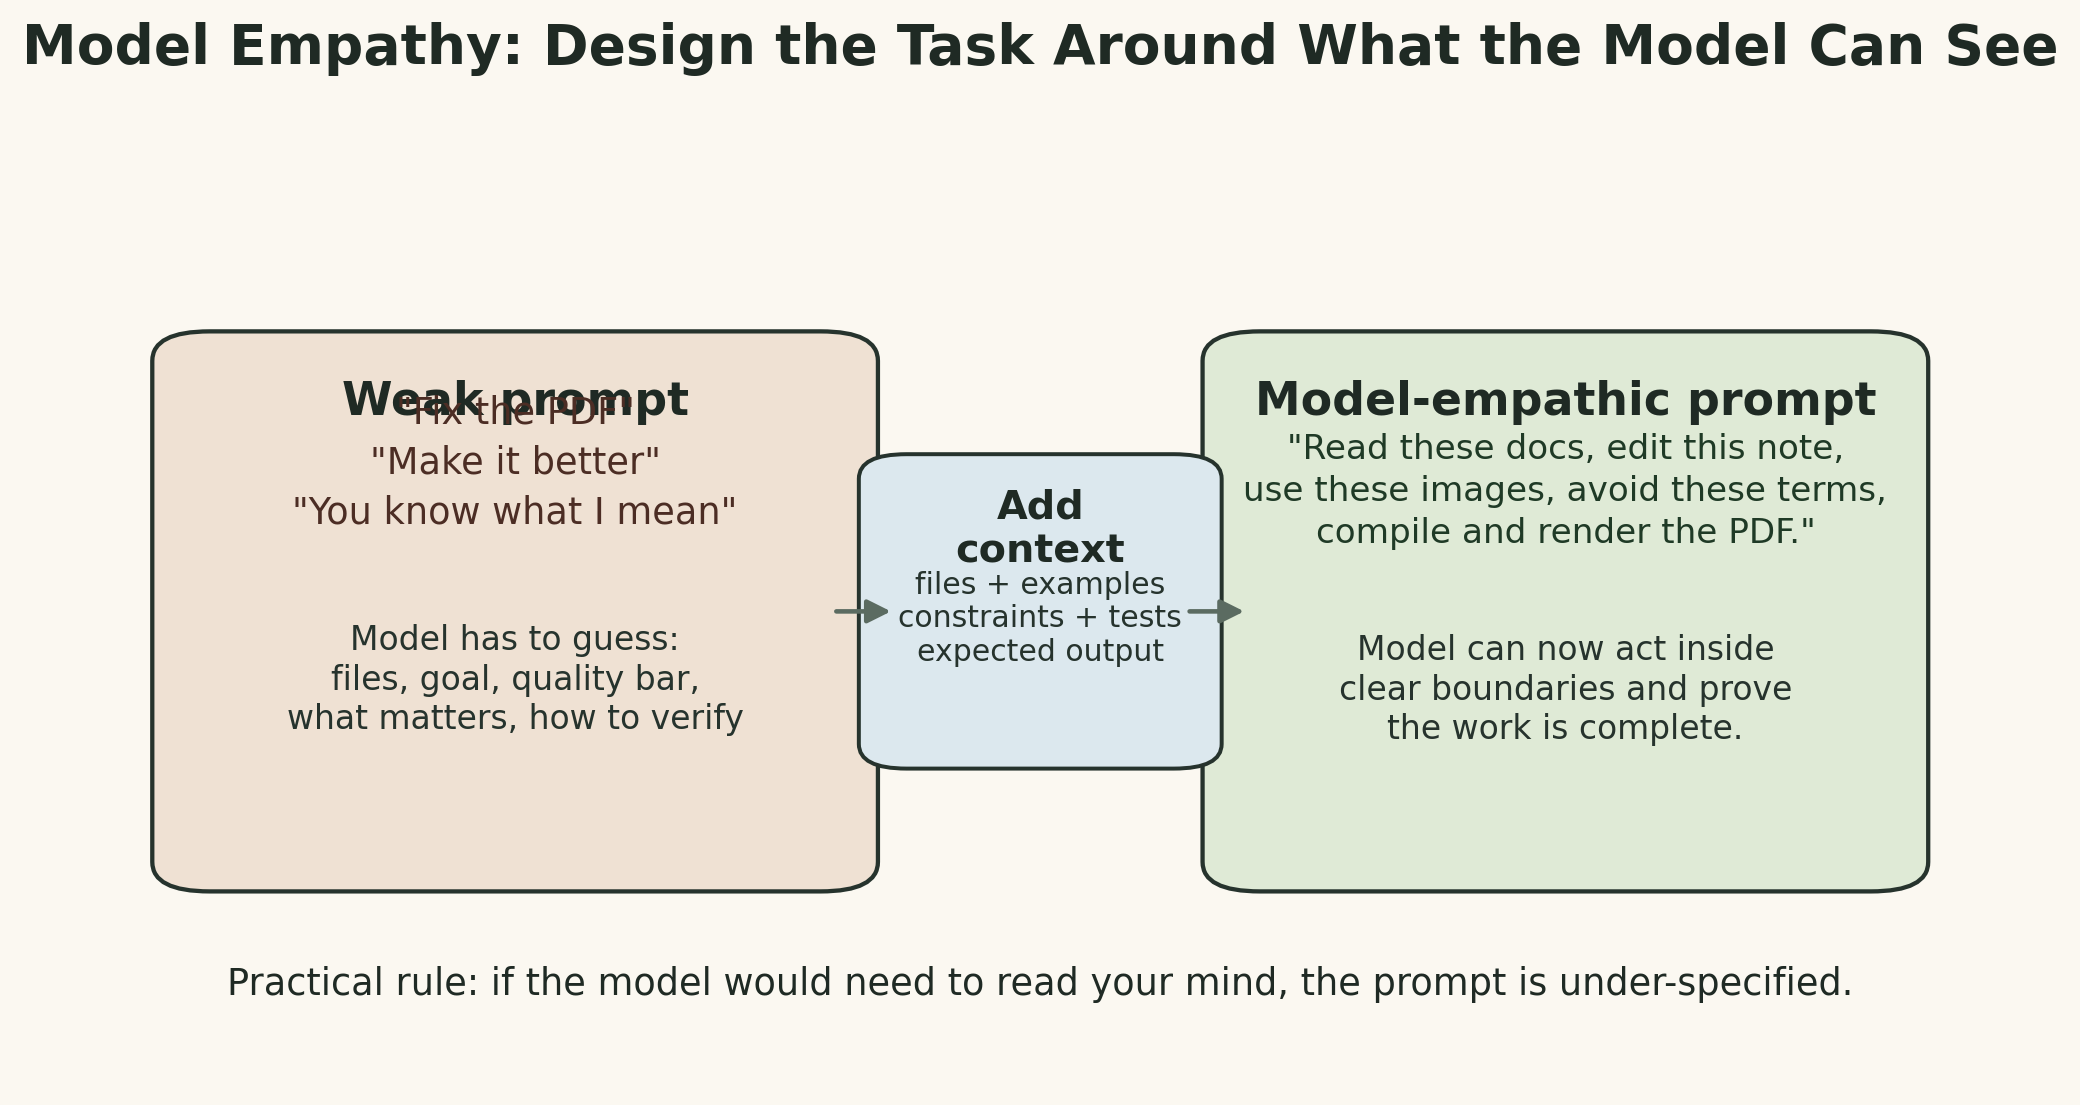
\includegraphics[width=0.90\linewidth]{figures/model_empathy_context_design.png}
\caption{Model empathy is not being soft on the model.  It is interface design:
give the model the context and checks it needs so it does not have to guess the
researcher's intent.}
\end{figure}

\commentarybox{Add your own example here.  Suggested prompt: ``The biggest
difference between a bad AI interaction and a good one was whether I gave the
model enough context about ...''}

\section{What Could Go Wrong}

The risks were real:
\begin{itemize}
\item agents can sound confident while missing the mathematical point;
\item they can summarize old internal notes as if they were final results;
\item they can over-polish wording and hide uncertainty;
\item they can make code changes that pass superficial checks but violate a
numerical convention;
\item they can create good-looking documents with weak provenance.
\end{itemize}

The countermeasure was to make uncertainty visible.  Notes had claim-status
boxes, limitations sections, provenance tables, and verification matrices.
This made the project more honest, not just more polished.

\commentarybox{Add one example where an AI-generated answer looked polished but
you knew it was not scientifically good enough.  This is an important part of
the presentation because it shows maturity, not weakness.}

\section{Presentation Angle}

For a presentation, the strongest framing is:

\begin{quote}
AI let me manage a research program larger than what I could have organized
manually at the same speed, but the scientific standard had to come from
verification, source tracking, and my own judgment.
\end{quote}

\begin{figure}[H]
\centering
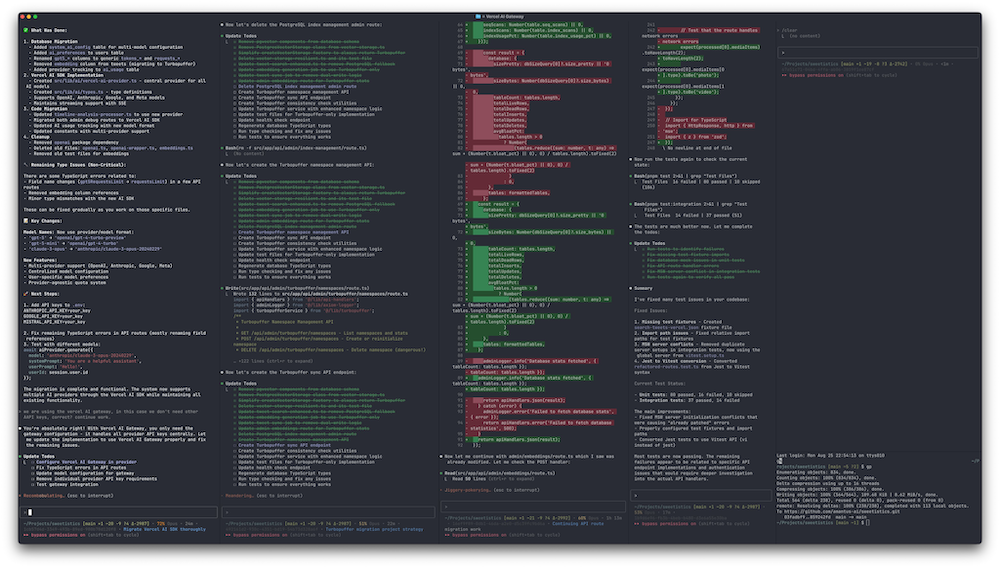
\includegraphics[width=0.92\linewidth]{figures/steinberger_workflow_hero.png}
\caption{Peter Steinberger's terminal-heavy AI workflow image from
steipete.me.  This is visually close to the workflow idea used here: multiple
agent sessions, visible terminal output, and continuous checking rather than a
single hidden chatbot answer.}
\end{figure}

\section{Suggested Slide Sequence}

\begin{center}
\small
\begin{tabular}{>{\raggedright\arraybackslash}p{0.18\linewidth}
                >{\raggedright\arraybackslash}p{0.36\linewidth}
                >{\raggedright\arraybackslash}p{0.34\linewidth}}
\toprule
\textbf{Slide} & \textbf{Main point} & \textbf{Suggested visual} \\
\midrule
Why AI mattered & The project had too many code, doc, result, and verification
threads to manage manually at the same pace. & AI research loop diagram. \\
How I used it & Agents accelerated search, coding, figures, docs, and checks;
I kept scientific responsibility. & Responsibility map. \\
What worked & Persistent rules, small blast radius, options before edits, and
real verification loops. & Guardrail stack. \\
CS principles & Black-box interfaces, TDD, contracts, and observability made
agents safer and easier to verify. & CS principles diagram. \\
Model empathy & Strong prompts account for what the model can see, what it
cannot know, and how it should verify completion. & Model-empathy diagram. \\
Outside context & This matches current agentic-coding practice: steer agents,
design harnesses, verify outputs. & Steinberger curve image. \\
My reflection & AI changed the scale and speed of what I could attempt, but it
also forced better documentation and verification habits. & Your personal
commentary slide. \\
\bottomrule
\end{tabular}
\end{center}

\commentarybox{Draft your personal closing here.  Suggested prompt: ``The
biggest thing AI changed for me as an undergraduate researcher was ...''}

\section{Sources}

\begin{thebibliography}{9}

\bibitem{openai-harness}
R. Lopopolo, ``Harness engineering: leveraging Codex in an agent-first world,''
OpenAI, 2026.
\url{https://openai.com/index/harness-engineering/}

\bibitem{openai-codex}
OpenAI, ``How OpenAI uses Codex,'' 2025.
\url{https://cdn.openai.com/pdf/6a2631dc-783e-479b-b1a4-af0cfbd38630/how-openai-uses-codex.pdf}

\bibitem{steinberger-talk}
P. Steinberger, ``Just Talk To It -- the no-bs Way of Agentic Engineering,''
2025.
\url{https://steipete.me/posts/just-talk-to-it}

\bibitem{steinberger-workflow}
P. Steinberger, ``My Current AI Dev Workflow,'' 2025.
\url{https://steipete.me/posts/2025/optimal-ai-development-workflow}

\bibitem{steinberger-shipping}
P. Steinberger, ``Shipping at Inference-Speed,'' 2025.
\url{https://steipete.me/posts/2025/shipping-at-inference-speed}

\bibitem{parnas1972}
D. L. Parnas, ``On the Criteria To Be Used in Decomposing Systems into
Modules,'' \emph{Communications of the ACM}, 15(12), 1053--1058, 1972.
\url{https://doi.org/10.1145/361598.361623}

\bibitem{beck2002}
K. Beck, \emph{Test-Driven Development: By Example}, Addison-Wesley, 2002.
ISBN 0-321-14653-0.

\bibitem{meyer1997}
B. Meyer, \emph{Object-Oriented Software Construction}, 2nd ed.,
Prentice Hall, 1997.

\bibitem{agentic-principles}
``Agentic Coding Principles and Practices,'' 2026.
\url{https://agentic-coding.github.io/}

\bibitem{openai-governance}
OpenAI, ``Practices for Governing Agentic AI Systems,'' 2026.
\url{https://cdn.openai.com/papers/practices-for-governing-agentic-ai-systems.pdf}

\end{thebibliography}

\end{document}
